\documentclass[11pt,titlepage,a4paper]{article}
\usepackage{setspace}

\usepackage[style=american]{csquotes}

\usepackage[backend=biber,style=numeric,sorting=none]{biblatex}
\addbibresource{bib.bib}

\usepackage{fancyhdr}
\setlength{\headheight}{14pt}
\pagestyle{fancy}

\lhead{}
\chead{Ramię robota}
\rhead{}
\lfoot{}
\cfoot{}
\rfoot{str. \thepage}

% Polski
\usepackage[]{polski} 
\usepackage[polish]{babel}

% Pierwszy akapit - wcięty
\usepackage[]{indentfirst}

% eps
\usepackage{graphicx}
\usepackage{subfigure}

\renewcommand*{\thesubsubsection}{}

\usepackage[dvipsnames]{xcolor}

\usepackage{hyperref}
\hypersetup{
    colorlinks,
    citecolor=black,
    filecolor=black,
    linkcolor=black,
    urlcolor=black
}

\usepackage{listings}
\usepackage{xcolor}
\lstset { %
    language=C++,
    basicstyle=\footnotesize\ttfamily,       
    breakatwhitespace=false,         
    breaklines=true,                 
    commentstyle=\color{gray},    
    extendedchars=true,              
    frame=single,                    
    keepspaces=true,                 
    keywordstyle=\color{orange},       
    numbers=left,                    
    numbersep=5pt,                   
    numberstyle=\footnotesize\color{gray}, 
    rulecolor=\color{black},         
    rulesepcolor=\color{blue},
    showspaces=false,                
    showstringspaces=false,          
    showtabs=false,                  
    stringstyle=\color{orange},    
    tabsize=2,                       
    emphstyle=\bfseries\color{blue}%  style for emph={} 
}

\hbadness = 1

\title{

\includegraphics[scale=0.75]{img/politechnika_sl_logo_bw_poziom_pl.eps}\\
\textbf{
Wydział Automatyki, Elektroniki i Informatyki}\\
\vspace*{1cm}
Projekt z Systemów Mikroprocesorowych\\
Ramię robota\\
}
% TODO Nie jestem pewnien sekcji
\author{Mateusz Siedliski i Radosław Tchórzewski\\
Rok akademicki 2022/2023, semestr 5, grupa 6, sekcja 2\\
\\
Kierujący pracą: dr inż. Jacek Loska} 
\date{Gliwice 2023}

\begin{document}

\onehalfspacing

\maketitle

\tableofcontents

\newpage

\section{\textcolor{blue}{DONE?} Wstęp}

Podczas studiowania na kierunku Automatyka i Robotyka można zauważyć zadziwiający brak fizycznych pomocy naukowych. Ten projekt ma na celu poprawę tej sytuacji choćby w niewielkim stopniu. W tym celu zaproponowano stworzenie ramienia robota (manipulatora). Ma on na celu pomoc studentom z wizualizacją koncepcji teoretycznych w prawdziwym świecie, a nie tylko w książkach, czy na ekranie komputera.

Projekt może posłużyć także do zachęcenia potencjalnych studentów podczas na przykład dni otwartych czy wycieczek szkolnych.

Główną inspiracją projektu był film zamieszczony na platformie YouTube z kanału \enquote{How To Mechatronics} pod tytułem \enquote{DIY Arduino Robot Arm with Smartphone Control} \cite*{HTM_YT}.

Nasz projekt korzysta z tych samych technologii, aczkolwiek wszystkie elementy (model 3D, oprogramowanie mikrokontrolera, kod aplikacji, schemat połączeń itd.) zostały przygotowane przez nas.

W ramach projektu stworzono dydaktyczny model 5 osiowego manipulatora z chwytakiem, zrealizowanego w technologii druku 3D, sterowany aplikacją na urządzenia z systemem Android.

\vspace*{2.5cm}

\subsection{\textcolor{blue}{DONE?} Cel i zakres projektu}

\subsubsection{\textcolor{blue}{DONE?} Cel projektu}

Celem projektu była realizacja fizycznego modelu manipulatora przeznaczonego do celów dydaktycznych. Może być on pomocny dla studentów w celu wizualizacji koncepcji teoretycznych w prawdziwym świecie, a nie tylko w książkach, czy na ekranie komputera.

Projekt może posłużyć także do zachęcenia potencjalnych studentów podczas na przykład dni otwartych czy wycieczek szkolnych.

\newpage

\subsubsection{\textcolor{blue}{DONE?} Wymagania}

\begin{itemize}
    \item Niski koszt budowy.
    \item Niski koszt eksploatacji.
    \item Stworzony z łatwodostępnych materiałów.
    \item Łatwość obsługi.
    \item Niski koszt szkolenia.
    \item Niska awaryjność.
    \item Łatwość naprawy.
    \item Atrakcyjny wygląd.
\end{itemize}

\vspace*{2.5cm}

\subsubsection{\textcolor{blue}{DONE?} Zakres projektu}

\begin{itemize}
    \item Określenie problemu i wykonanie do niego założeń.
    \item Analiza możliwych rozwiązań.
    \item Wybór elementów elektronicznych.
    \item Wybór elementów mechanicznych.
    \item Wykonanie projektu zgodnie z wcześniejszymi założeniami.
    \item Uruchomienie, weryfikacji i przetestowanie sprzętu i aplikacji.
    \item Nakreślenie ewentualnych kierunków rozwoju projektu.
    \item Wnioski końcowe.
\end{itemize}

\newpage

\section{\textcolor{blue}{DONE?} Harmonogram}

\subsection{\textcolor{green}{DONE} Harmonogram zatwierdzony}

\begin{enumerate}
    \item Projektowanie modelu fizycznego robota oraz jego druk w technologii 3D.
    \item Montaż mechaniczny oraz elektryczny.
    \item Tworzenie oprogramowania na mikrokontroler.
    \item Tworzenie aplikacji sterującej.
    \item Projektowanie oraz realizacja komunikacji między mikrokontrolerem, \\a aplikacją sterującą.
\end{enumerate}

\vspace*{2.5cm}

\subsection{\textcolor{blue}{DONE?} Harmonogram wykonany}

Realizacja działającego prototypu zajęła zdecydowanie mniej czasu, niż początkowo zakładano. Pozwoliło to na poświęcenie większej ilości czasu na uprawnienia i udoskonalanie projektu.

\begin{enumerate}
    \item Projektowanie modelu fizycznego robota oraz jego druk w technologii 3D. Montaż mechaniczny oraz elektryczny.
    \item Tworzenie oprogramowania na mikrokontroler oraz aplikacji sterującej. Opracowanie protokołu komunikacji między mikrokontrolerem, a aplikacją sterującą.
    \item Doskonalenie projektu — debugowanie, poprawki mechaniczne, usprawnienia
    \item Doskonalenie projektu — debugowanie, poprawki mechaniczne, usprawnienia
    \item Doskonalenie projektu — debugowanie, poprawki mechaniczne, usprawnienia
\end{enumerate}

\newpage

\section{\textcolor{blue}{DONE?} Kosztorys}

\begin{center}
    \begin{tabular}{|r|l|l|c|r|r|}
        \hline
        Lp. & Typ                          & Producent & Ilość & Cena     & Wartość  \\
        \hline
        1.  & Mikrokontroler Wemos D1 mini & Wemos     & 1     & 9,48 zł  & 9,48 zł  \\
        2.  & Moduł Bluetooth HC-05        & SZYTF     & 1     & 9,40 zł  & 9,40 zł  \\
        3.  & Micro Servo 9g SG90          & HWAYEH    & 3     & 3,97 zł  & 11,91 zł \\
        4.  & Servo Mg996r                 & WAVGAT    & 3     & 12 zł    & 36 zł    \\
        5.  & Obudowa ramienia (druk 3D)   & n/d       & 1     & 40 zł    & 40 zł    \\
        6.  & Przewody                     & n/d       & n/d   & n/d      & 10 zł    \\
        7.  & Płytka prototypowa           & diymore   & 1     & 3,15 zł  & 3,15 zł  \\
        8.  & Wkręty M3                    & n/d       & 4     & 0,20 zł  & 0,80 zł  \\
        9.  & Śruby M3                     & n/d       & 8     & 0,20 zł  & 1,60 zł  \\
        10. & Nakrętki M3                  & n/d       & 18    & 0,20 zł  & 3,60 zł  \\
        11. & Drewniana podstawa           & n/d       & 1     & 10,00 zł & 10,00 zł \\
        12. & Kondensator $1000\ \mu F$    & Chong     & 1     & 0,50 zł  & 0,50 zł  \\
        \hline
        \multicolumn{6}{|r|}{Suma = 136,44 zł}                                       \\
        \hline
        \multicolumn{6}{|r|}{Ilość roboczogodzin = 40}                               \\
        \hline
    \end{tabular}
\end{center}

\newpage

\section{\textcolor{orange}{TODO} Urządzenie wraz z aplikacją}

Należy podać krótki opis celu który chcemy osiągnąć wykonując projekt.
Pozostałe punkty mają ułatwić napisanie projektu, ale nie są bezwzględnie wymagane. Powinno się je elastycznie dopasować do zrealizowanego projektu – SZCZEGÓLNIE nazwy podrozdziałów.
Ta część powinna zwierać od 20 do 25 stron.

\subsection{\textcolor{orange}{TODO} Określenie problemu}

Dokładne opisanie problemu. Wykonać schematy ideowe i blokowe, dołączyć ilustrujące problem rysunki itp. Wykonać założenia potrzebne do rozwiązania postawionego problemu.

Rysunek 1. To jest rysunek podstawowego bloku systemu.

Należy zawsze odwoływać się do tego co jest na Rysunek 1.

\subsection{\textcolor{orange}{TODO} Analiza rozwiązań}

W tym punkcie powinno się przedstawić jakie są możliwości rozwiązania problemu (urządzenia, technologie i produkty), wraz z określeniem kryteriów wyboru rozwiązania.

\subsection{\textcolor{orange}{TODO} Zaproponowane rozwiązanie}

W tym punkcie należy przedstawić wybrane rozwiązanie problemu, wraz z uzasadnieniem wyboru na postawie kryteriów z poprzedniego punktu.

\subsection{\textcolor{orange}{TODO} Wykonanie}

W tym punkcie opisać jak zostało wykonane urządzenie oraz zaprogramowana aplikacja, jakie zastosowano technologie, narzędzia do pisania, weryfikowania i testowania aplikacji. Nie należy umieszczać kodu programu, jedynie wybrane fragmenty pokazujące rozwiązanie niestandardowego problemu. Pełny kod programu należy przesłać emailem ew. dodatkowo umieścić w załączniku.
Jest to najważniejszy punkt w projekcie – proszę mu poświęcić jak najwięcej uwagi minimum 15-18 stron!!!

\subsection{\textcolor{orange}{TODO} Problemy w trakcie tworzenia sprzętu i aplikacji (niepotrzebne usunąć!)}

W tym punkcie należy przedstawić jakie były problemy przed którymi stanęli autorzy projektu w trakcie jego realizacji i jak je rozwiązali.

\newpage

\section{\textcolor{orange}{TODO} Podsumowanie}

W ostatnim punkcie opisać co zostało wykonane, jakiej części założeń nie wykonano i dlaczego. Co można zrobić, by dany projekt poprawić i w jakim kierunku może pójść dalszy rozwój tego projektu.

\newpage

\section{\textcolor{red}{WIP}  Literatura}

\printbibliography[heading=none]

\newpage

\section{\textcolor{orange}{TODO} Załączniki}

Na prezentację (obronę) projektu trzeba przygotować prezentację w PowerPoint lub Prezi trwającą ok 12-15 minut Zwykle jest to ok. 20 slajdów. Te slajdy muszą zawierać tytuł projektu, autora, prowadzącego. Następnie plan prezentacji, najważniejsze osiągnięcia , podsumowanie. Slajdy muszą być czytelne, należy umieszczać rysunki i schematy, także nie powinno się na nich umieszczać zbyt dużo tekstu (tekst powinien mieć ok. 20-24pkt). W trakcie lub po prezentacji powinno się zademonstrować wykonany sprzęt i oprogramowanie. Można również zaprezentować w zamian tego film z działania urządzenia.

Przykładowa zawartość załącznika:
Kody źródłowe (z komentarzami!!!) na CD spakowane.
Wysłane mailem zawartość projektu do prowadzącego.
Prezentacja.
Wszystkie opisy układów, programów, narzędzi stosowanych w projekcie itp.

\newpage

\section{Kod}

\subsection{Kod mikrokontrolera}

\lstinputlisting[]{../src/main.cpp}

\subsection{Kod aplikacji}

\subsubsection{Bluetooth}

\begin{center}
    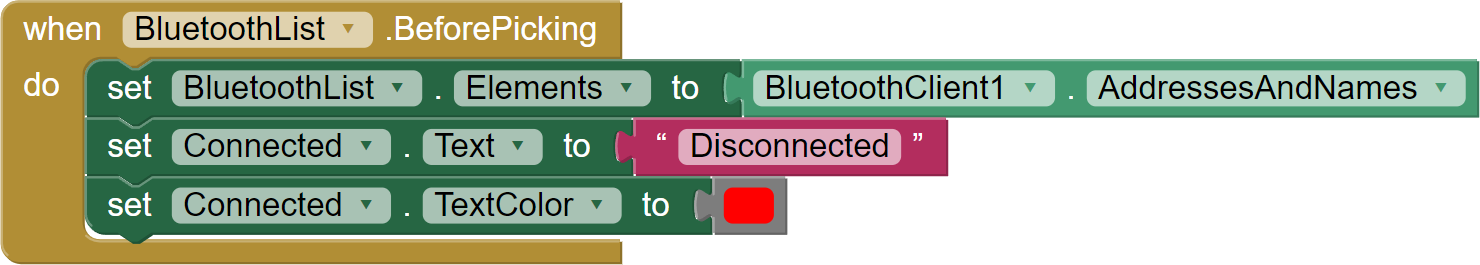
\includegraphics[width=0.8\textwidth]{img/app_src/bluetooth/BluetoothListBefore.png}
    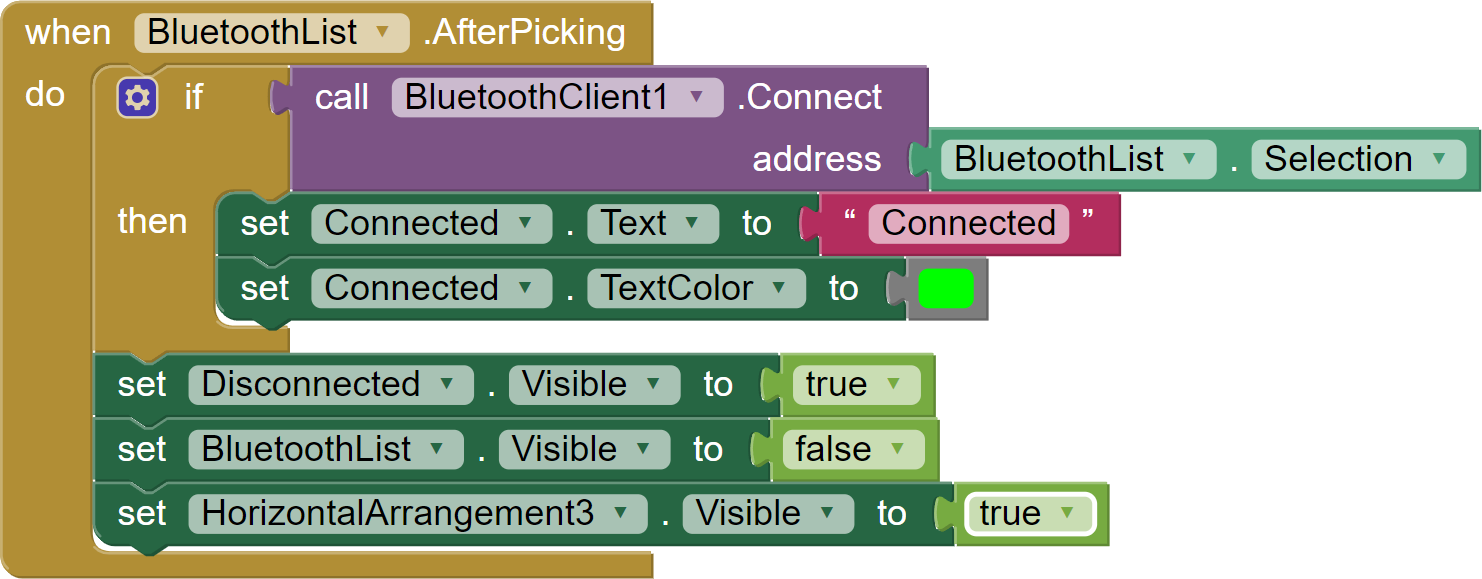
\includegraphics[width=0.8\textwidth]{img/app_src/bluetooth/BluetoothListAfter.png}
    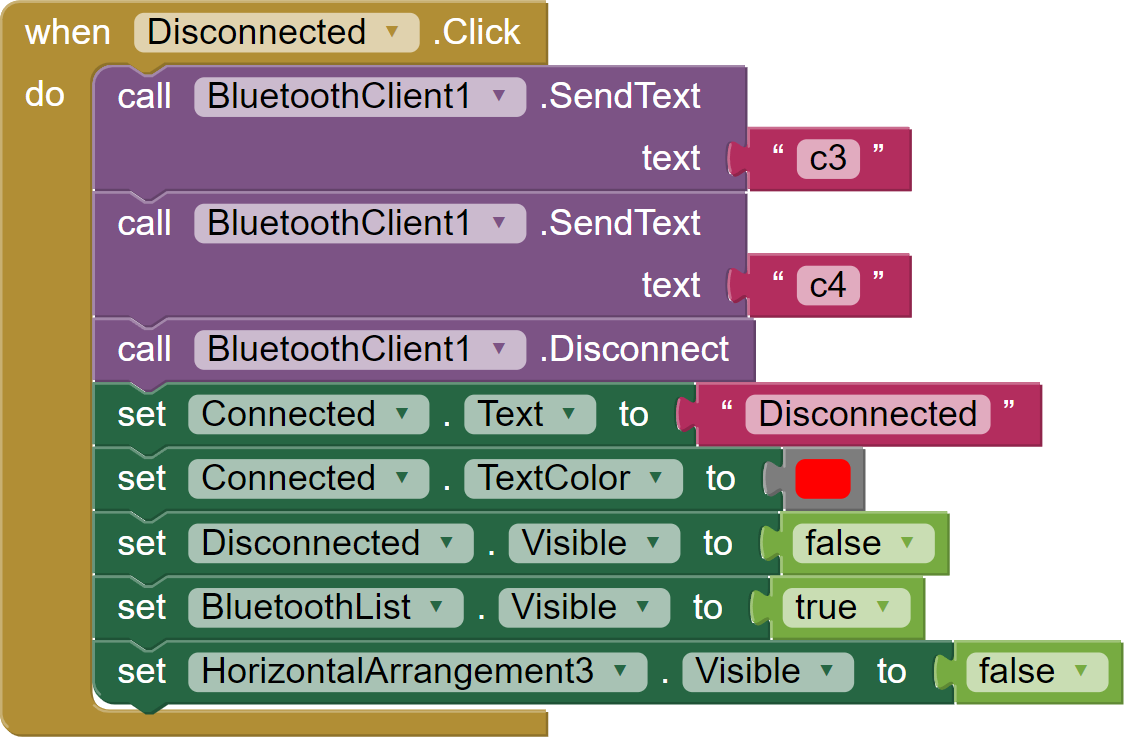
\includegraphics[width=0.8\textwidth]{img/app_src/bluetooth/BluetoothDisconnected.png}
    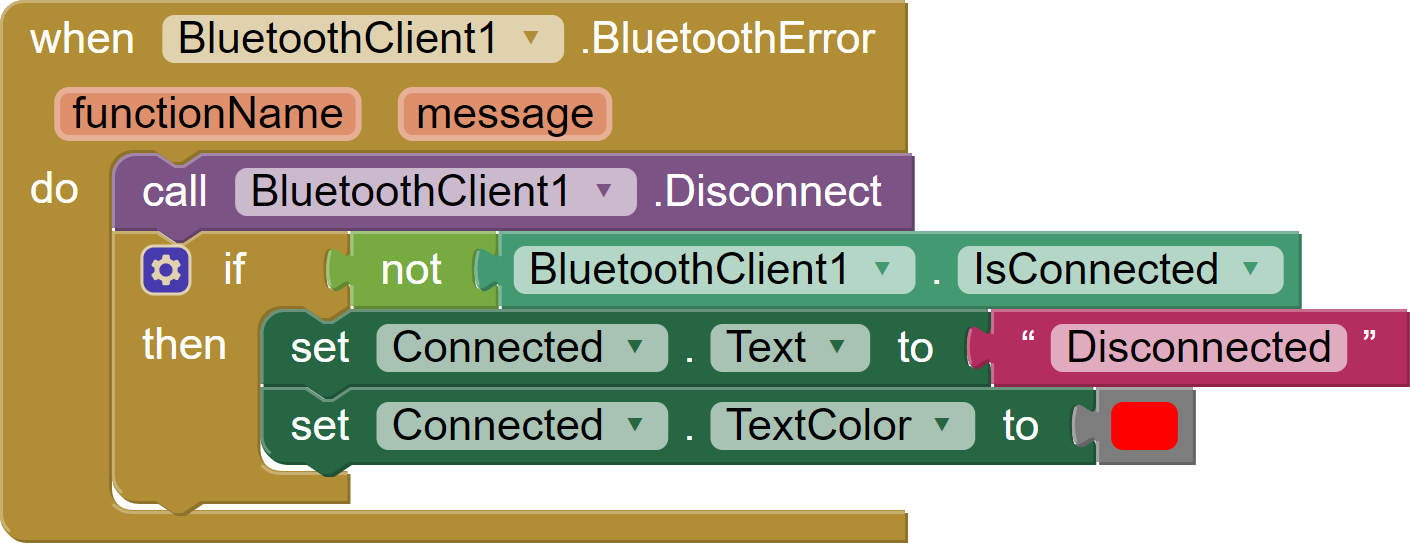
\includegraphics[width=0.8\textwidth]{img/app_src/bluetooth/BluetoothClient.png}
\end{center}

\newpage

\subsubsection{Przyciski}

\begin{center}
    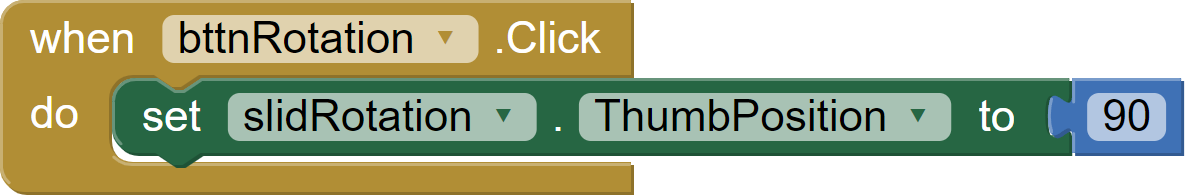
\includegraphics[width=0.9\textwidth]{img/app_src/posButtons/bttnRotation.png}
    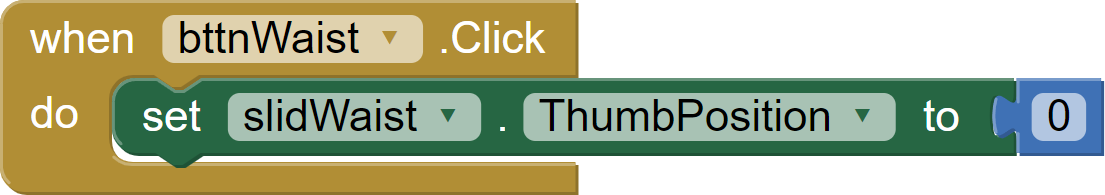
\includegraphics[width=0.9\textwidth]{img/app_src/posButtons/bttnWaist.png}
    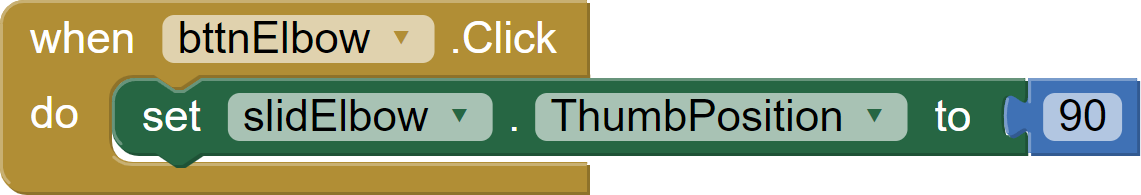
\includegraphics[width=0.9\textwidth]{img/app_src/posButtons/bttnElbow.png}
    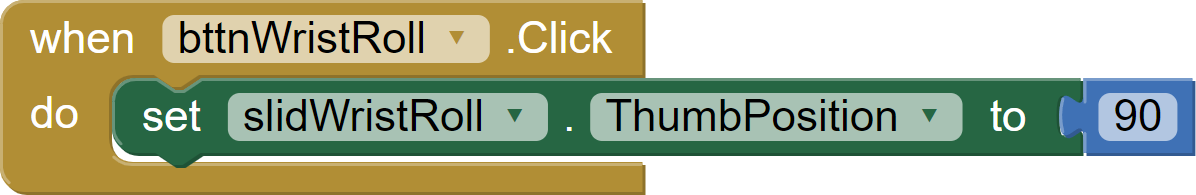
\includegraphics[width=0.9\textwidth]{img/app_src/posButtons/bttnWristRoll.png}
    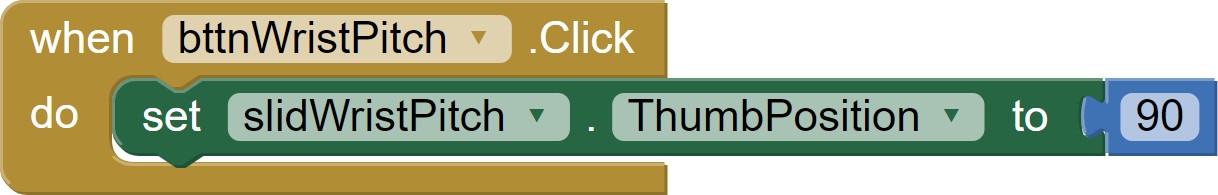
\includegraphics[width=0.9\textwidth]{img/app_src/posButtons/bttnWristPitch.png}
    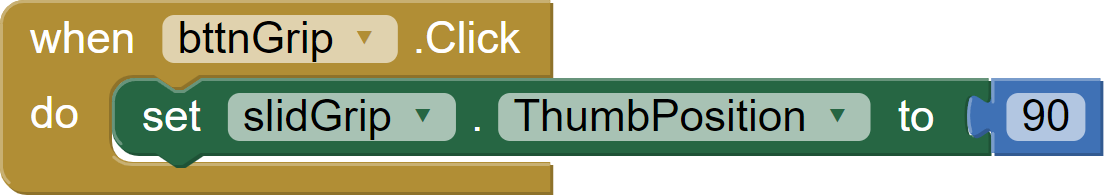
\includegraphics[width=0.9\textwidth]{img/app_src/posButtons/bttnGrip.png}
\end{center}

\newpage

\subsubsection{Slidery}

\begin{center}
    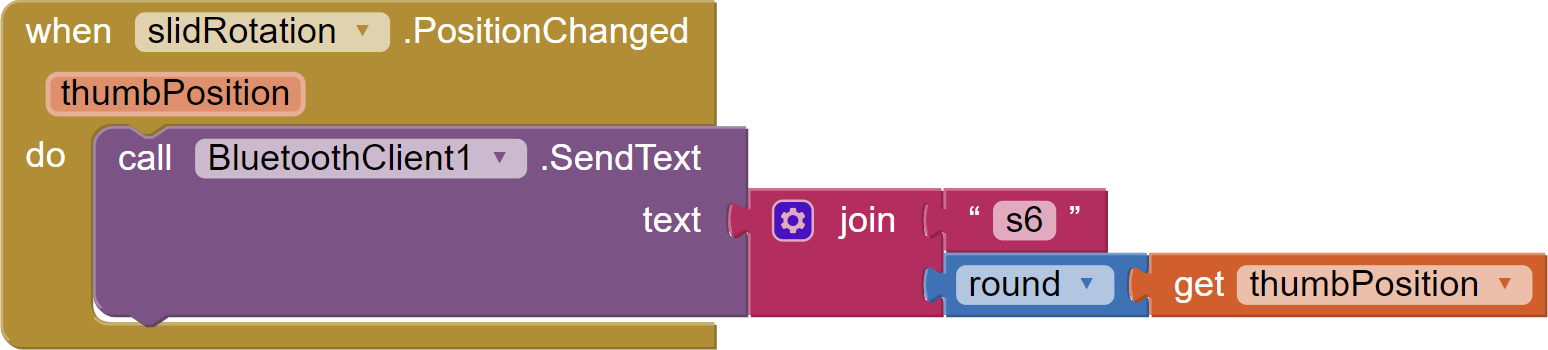
\includegraphics[width=0.9\textwidth]{img/app_src/sliders/slidRotation.png}
    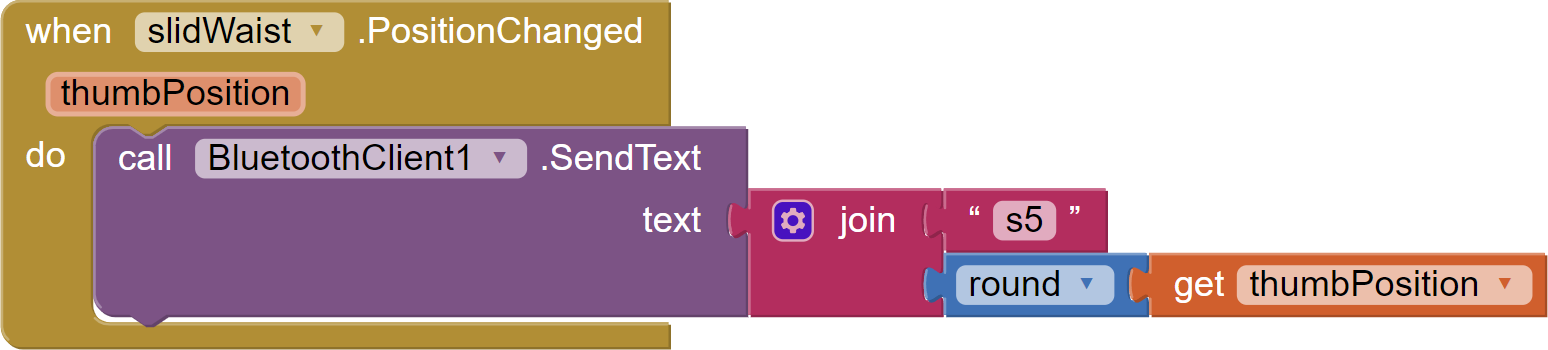
\includegraphics[width=0.9\textwidth]{img/app_src/sliders/slidWaist.png}
    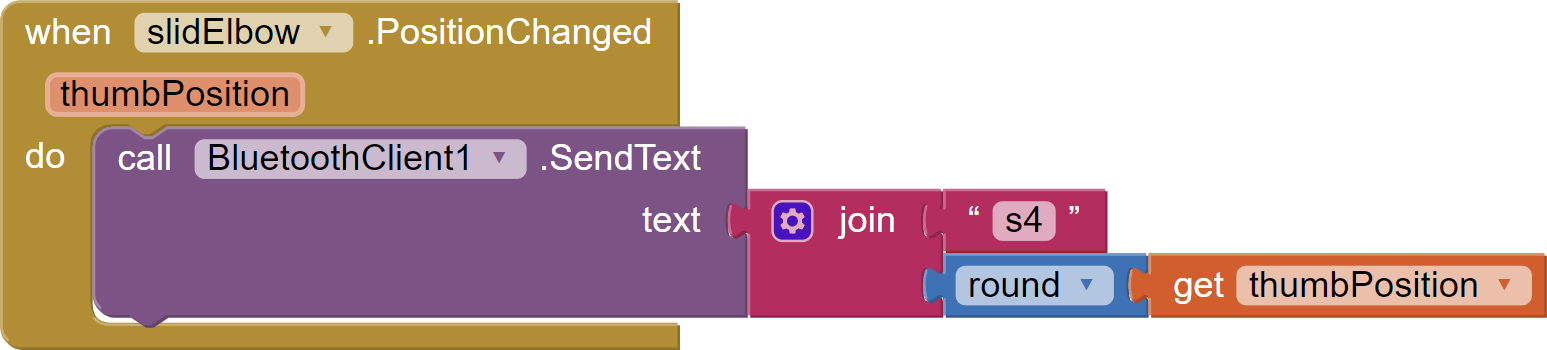
\includegraphics[width=0.9\textwidth]{img/app_src/sliders/slidElbow.png}
    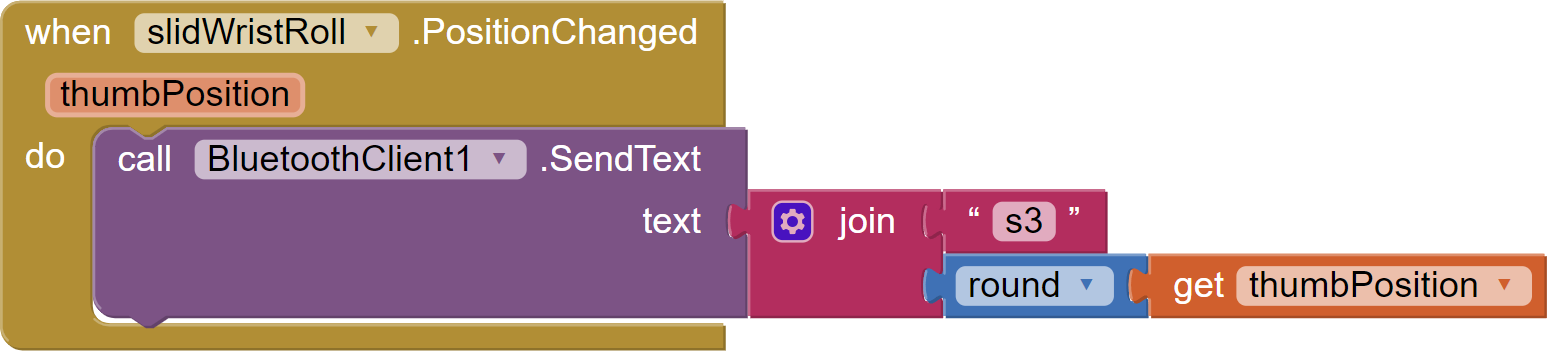
\includegraphics[width=0.9\textwidth]{img/app_src/sliders/slidWristRoll.png}
    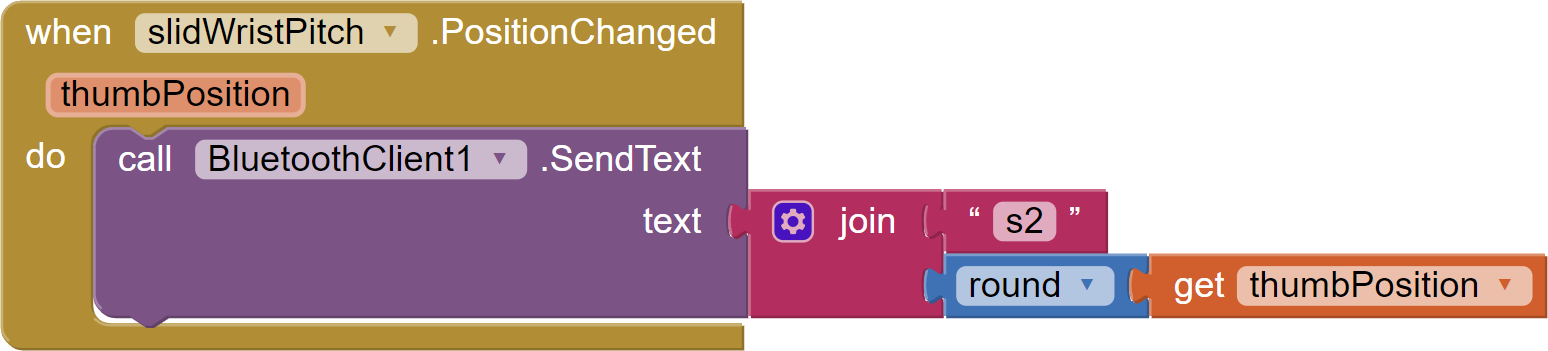
\includegraphics[width=0.9\textwidth]{img/app_src/sliders/slidWristPitch.png}
    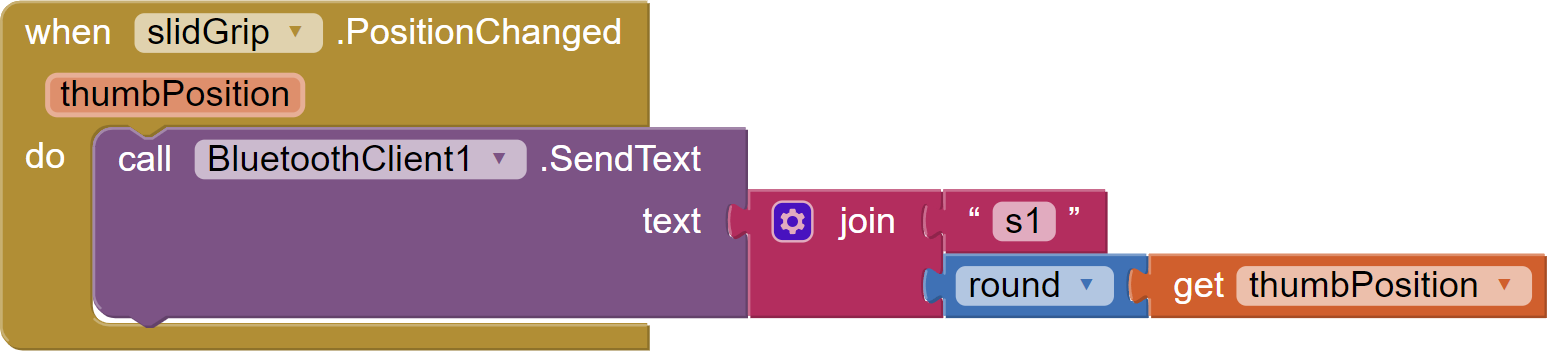
\includegraphics[width=0.9\textwidth]{img/app_src/sliders/slidGrip.png}
\end{center}

\newpage

\subsubsection{Komendy}

\begin{center}
    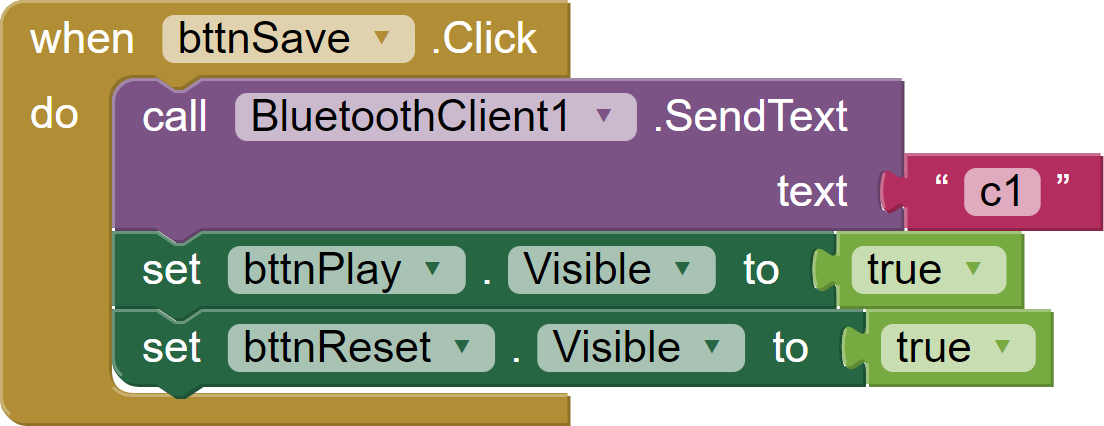
\includegraphics[width=0.8\textwidth]{img/app_src/commands/Save.png}
    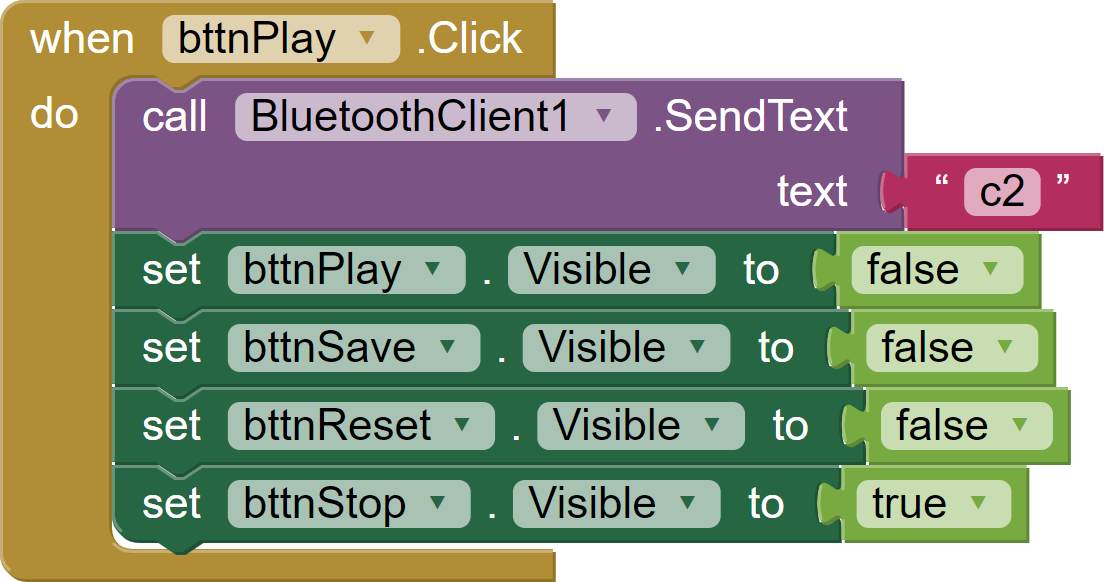
\includegraphics[width=0.8\textwidth]{img/app_src/commands/Play.png}
    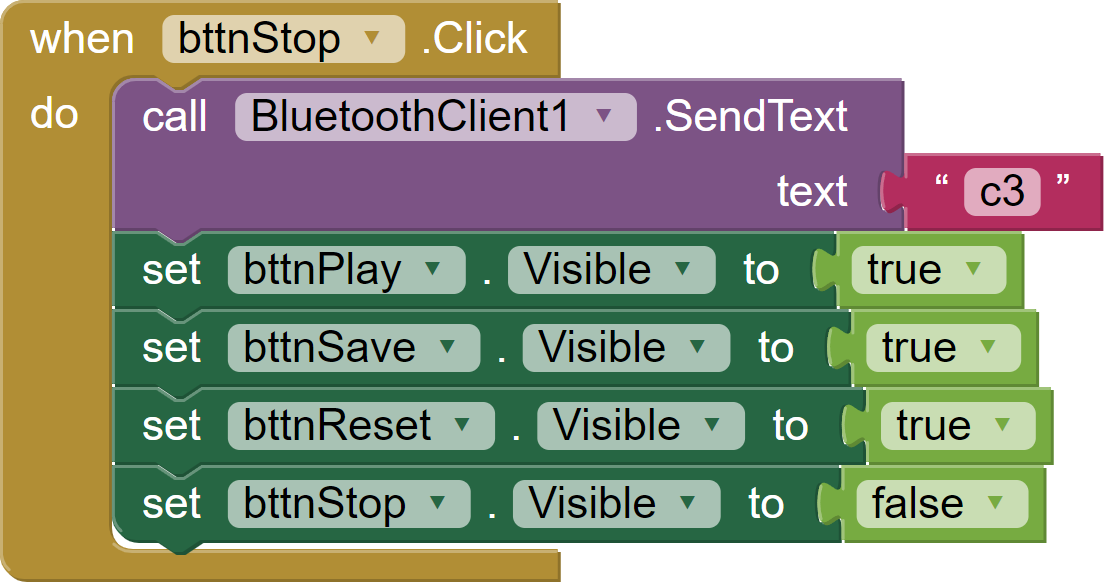
\includegraphics[width=0.8\textwidth]{img/app_src/commands/Stop.png}
    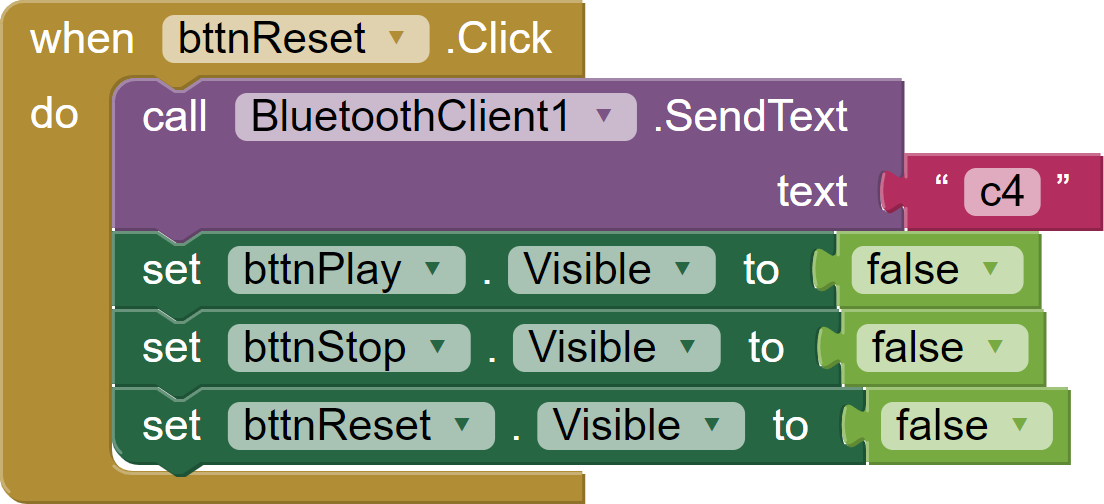
\includegraphics[width=0.8\textwidth]{img/app_src/commands/Reset.png}
\end{center}

\end{document}